%%%%%%%%%%%%%%%%%%%%%%%%%%%%%%%%%%%%%%%%%%%%%%%%%%%%%%%%%%%%%%%%%%%%%%%%%%%%%%%%%%%%%%%%%%%%%%%%%%%%%%%%%%%%%%%%%%%%%%%%%%%%%%%%%%%%%%%%%%%%%%%%%%%%%%%%%%%%%%%%%%%
% Written By Michael Brodskiy
% Class: Fundamentals of Linear Systems
% Professor: I. Salama
%%%%%%%%%%%%%%%%%%%%%%%%%%%%%%%%%%%%%%%%%%%%%%%%%%%%%%%%%%%%%%%%%%%%%%%%%%%%%%%%%%%%%%%%%%%%%%%%%%%%%%%%%%%%%%%%%%%%%%%%%%%%%%%%%%%%%%%%%%%%%%%%%%%%%%%%%%%%%%%%%%%

\include{Includes.tex}

\title{Homework 3}
\date{\today}
\author{Michael Brodskiy\\ \small Professor: I. Salama}

\begin{document}

\maketitle

\begin{enumerate}

  \item Classifying systems as memory-less, time-invariant, linear, causal, and/or stable:

    \begin{enumerate}

      \item $y(t)=5e^{4t}x(t-1)$

        \begin{itemize}

          \item Memory: \textbf{not} memory-less; the $x(t-1)$ term means the system relies on values other than the present value; therefore, it is not memory-less

          \item Time-Invariant: \textbf{not} time-invariant; we may see that, $y(t-t_o)$ changes the $t$ value in the exponential and $x(t)$ statement, while $x(t-t_o)$ changes only the $x(t)$ statement; thus, it is not time-invariant, since $x(t-t_o)\neq y(t-t_o)$

          \item Linear: the system \textbf{is} linear (see below) because $ax_1(t)+bx_2(t)= ay_1(t)+by_2(t)$

            $$ax_1(t)+bx_2(t)\to a5e^{4t}x_1(t-1)+b5e^{4t}x_2(t-1)$$
            $$ay_1(t)+by_2(t)\to a5e^{4t}x_1(t-1)+b5e^{4t}x_2(t-1)$$

          \item Causal: the system \textbf{is} causal , because it only depends on past or present values (ex. $t=0\to y(t)=5e^{4(0)}x(-1)$)

          \item Stable: Given that the system depends on an exponential $e^{4t}$, its maximum value is unbounded and, therefore, it is \textbf{unstable}

        \end{itemize}

      \item $y(t)=\displaystyle \int_{-\infty}^{\frac{t}{2}} x(\tau)\,d\tau$

        \begin{itemize}

          \item Memory: \textbf{not} memory-less; the system depends on a shift of the $t$ parameter ($t/2$), and, therefore, does not always depend on the current value of time

          \item Time-Invariant: \textbf{not} time-invariant; $y(t-t_o)\neq x(t-t_o)$ (see below)

            $$x(t-t_o)\to \int_{-\infty}^{\frac{t}{2}} x(\tau-t_o)\,d\tau$$
            $$y(t-t_o)\to \int_{-\infty}^{\frac{(t-t_o)}{2}} x(\tau-t_o)\,d\tau$$
            $$\therefore x(t-t_o)\neq y(t-t_o)$$

          \item Linear: the system \textbf{is} linear; it follows both the superposition and homogeneity principles (see below)

            $$ay_1(t)+by_2(t)\to a\int_{-\infty}^{\frac{t}{2}} x_1(\tau)\,d\tau+b\int_{-\infty}^{\frac{t}{2}} x_2(\tau)\,d\tau$$
            $$ax_1(t)+bx_2(t)\to a\int_{-\infty}^{\frac{t}{2}} x_1(\tau)\,d\tau+b\int_{-\infty}^{\frac{t}{2}} x_2(\tau)\,d\tau$$
            $$\therefore ax_1(t)+bx_2(t)=ay_1(t)+by_2(t)$$

          \item Causal: the system \textbf{is not} causal; integration depends on future values when $t<0$

          \item Stable: the system \textbf{is not} stable (see below)

            $$y(t)=\int_{-\infty}^{\frac{t}{2}} x(\tau)\,d\tau$$
            $$h(t)=\int_{-\infty}^{\frac{t}{2}} \delta(\tau)\,d\tau=\left\{\begin{array}{ll}0,& t<0\\1,& t>0\end{array}$$
            $$h(t)\to u(t)$$
            $$\int_{-\infty}^{\infty} h(t)\,dt=\infty$$

        \end{itemize}

      \item $y(t)=4+5\dfrac{d^2}{dt^2}x(t)$

        \begin{itemize}

          \item Memory: the system is \textbf{not} memory-less; the use of a differential implies that the system depends on past values

          \item Time-Invariant: the system \textbf{is} time-invariant (see below)

            $$x(t-t_o)\to 4+5\dfrac{d^2}{dt^2}x(t-t_o)$$
            $$y(t-t_o)\to 4+5\dfrac{d^2}{dt^2}x(t-t_o)$$
            $$\therefore x(t-t_o)=y(t-t_o)$$

          \item Linear: the system is \textbf{not} linear (see below)

            $$ax_1(t)+bx_2(t)=\left(4+5a\dfrac{d^2}{dt^2}x_1(t)\right)+\left(4+5b\dfrac{d^2}{dt^2}x_2(t)\right)$$
            $$ay_1(t)+by_2(t)=a\left(4+5\dfrac{d^2}{dt^2}x_1(t)\right)+b\left(4+5\dfrac{d^2}{dt^2}x_2(t)\right)$$
            $$\therefore ax_1(t)+bx_2(t)\neq ay_1(t)+by_2(t)$$

          \item Causal: the system \textbf{is} causal because it only depends on past or present values

          \item Stable: the system is \textbf{unstable} because it is unbounded

        \end{itemize}

      \item $y(t)=\left\{\begin{array}{ll} 0, & t<0\\ x(t-2)+2x(t), & t\geq0\end{array}$

        \begin{itemize}

          \item Memory: the system is \textbf{not} memory-less, since the $x(t-2)$ term depends on a past value

          \item Time-Invariant: the system is \textbf{not} time-invariant (see below)

            $$x(t-t_o)\to\left\{\begin{array}{ll} 0, & t<0\\ x(t-2-t_o)+2x(t-t_o), & t\geq0\end{array}$$
            $$y(t-t_o)\to\left\{\begin{array}{ll} 0, & t<2\\ x(t-2-t_o)+2x(t-t_o), & t\geq2\end{array}$$
            $$\therefore x(t-t_o)\neq y(t-t_o)$$

          \item Linear: the system \textbf{is} linear (see below)

            $$ax_1(t)+bx_2(t)\to\left\{\begin{array}{ll} 0, & t<0\\ ax_1(t-2)+2ax_1(t)+bx_2(t-2)+2bx_2(t), & t\geq0\end{array}$$
            $$ay_1(t)+by_2(t)\to\left\{\begin{array}{ll} 0, & t<0\\ ax_1(t-2)+2ax_1(t)+bx_2(t-2)+2bx_2(t), & t\geq0\end{array}$$
              $$\therefore ax_1(t)+bx_2(t)=ay_1(t)+by_2(t)$$

            \item Causal: the system \textbf{is} causal because it only depends on past or present values

            \item Stable: the system \textbf{is} stable, because it does not tend to diverge

        \end{itemize}

        Problem 1 can be tabulated as follows:

        \begin{center}
          \begin{tabular}[H]{|c|c|c|c|c|}
            \hline
            System & a & b & c & d\\
            \hline
            Memory-Less & no & no & no & no\\
            \hline
            Time-Invariant & no & no & yes & no\\
            \hline
            Linear & yes & yes & no & yes\\
            \hline
            Causal & yes & no & yes & yes\\
            \hline
            Stable & no & no & no & yes\\
            \hline
          \end{tabular}
        \end{center}

    \end{enumerate}

  \item Classifying systems as memory-less, time-invariant, linear, causal, and/or stable:

    \begin{enumerate}

      \item $y[n]=x[n+1]-2x[n-4]$

        \begin{itemize}

          \item Memory: system is \textbf{not} memory-less, as it depends on past and future values

          \item Time-Invariant: system \textbf{is} time-invariant (see below)

            $$x[n-n_o]=x[n+1-n_o]-2x[n-4-n_o]$$
            $$y[n-n_o]=x[n+1-n_o]-2x[n-4-n_o]$$
            $$\therefore x[n-n_o]=y[n-n_o]$$

          \item Linear: system \textbf{is} linear (see below)

            $$ax_1[n]+bx_2[n]=a(x_1[n+1]-2x_1[n-4])+b(x_2[n+1]-2x_2[n-4])$$
            $$ay_1[n]+by_2[n]=a(x_1[n+1]-2x_1[n-4])+b(x_2[n+1]-2x_2[n-4])$$
            $$\therefore ay_1[n]+by_2[n]=ax_1[n]+bx_2[n]$$

          \item Causal: system is \textbf{not} causal, as it depends on past and present values

          \item Stable: system \textbf{is} stable because $y[n]$ is finite

        \end{itemize}

      \item $y[n]=\text{Even}\left\{ x[n-1] \right\}$

        To simplify analysis, we can express the even function as:

        $$\frac{x[n]+x^*[-n]}{2}\to\frac{x[n-1]+x^*[-n+1]}{2}$$

        \begin{itemize}

          \item Memory: system is \textbf{not} memory-less, as it depends on future values

          \item Time-Invariant: system \textbf{is} time-invariant (see below)

            $$x[n-n_o]=\text{Even}\left\{ x[n-1-n_o] \right\}$$
            $$y[n-n_o]=\text{Even}\left\{ x[n-1-n_o] \right\}$$
            $$\therefore x[n-n_o]=y[n-n_o]$$

          \item Linear: system is \textbf{not} linear (see below); note that this is because $a$ or $b$ may be complex. Given this, for a purely real signal, the system can be classified as linear; however, due to the need to use the 'conjugate' for the even function, in the case of a complex signal, this is non-linear

            $$ax_1[n]+bx_2[n]=\frac{ax_1[n-1]+a^*x_1^*[-n+1]}{2}+\frac{bx_2[n-1]+b^*x_2^*[-n+1]}{2}$$
            $$ay_1[n]+by_2[n]=\frac{ax_1[n-1]+ax_1^*[-n+1]}{2}+\frac{bx_2[n-1]+bx_2^*[-n+1]}{2}$$
            $$\therefore ay_1[n]+by_2[n]\neq ax_1[n]+bx_2[n]$$

          \item Causal: system is \textbf{not} causal, as it depends on a future value

          \item Stable: system \textbf{is} stable because $y[n]$ is finite

        \end{itemize}

      \item $y[n]=5x[3n+1]$

        \begin{itemize}

          \item Memory: system is \textbf{not} memory-less, as it depends on non-present values

          \item Time-Invariant: system is \textbf{not} time-invariant (see below)

            $$x[n-n_o]=5x[3n-n_o+1]$$
            $$y[n-n_o]=5x[3n-3n_o+1]$$
            $$\therefore x[n-n_o]\neq y[n-n_o]$$

          \item Linear: system \textbf{is} linear (see below)

            $$ax_1[n]+bx_2[n]=5ax_1[3n+1]+5bx_2[3n+1]$$
            $$ay_1[n]+by_2[n]=5ax_1[3n+1]+5bx_2[3n+1]$$
            $$\therefore ay_1[n]+by_2[n]=ax_1[n]+bx_2[n]$$

          \item Causal: system is \textbf{not} causal, as it depends on a future value

          \item Stable: system \textbf{is} stable because $y[n]$ is finite

        \end{itemize}

      \item $y[n]=\left\{ \begin{array}{ll} 0, & n=2\\ x[n], & \text{otherwise}\end{array}$

        \begin{itemize}

          \item Memory: system \textbf{is} memory-less; it does not depend on past or present values

          \item Time-Invariant: system is \textbf{not} time-invariant (see below)

            $$x[n-n_o]=\left\{ \begin{array}{ll} 0, & n=2\\ x[n-n_o], & \text{otherwise}\end{array}$$
            $$y[n-n_o]=\left\{ \begin{array}{ll} 0, & n=2+n_o\\ x[n-n_o], & \text{otherwise}\end{array}$$
            $$\therefore x[n-n_o]\neq y[n-n_o]$$

          \item Linear: system \textbf{is} linear (see below)

            $$ax_1[n]+bx_2[n]=\left\{ \begin{array}{ll} 0, & n=2\\ ax_1[n]+bx_2[n], & \text{otherwise}\end{array}$$
            $$ay_1[n]+by_2[n]=\left\{ \begin{array}{ll} 0, & n=2\\ ax_1[n]+bx_2[n], & \text{otherwise}\end{array}$$
            $$\therefore ay_1[n]+by_2[n]=ax_1[n]+bx_2[n]$$

          \item Causal: system \textbf{is} causal, as it depends on only past or present values

          \item Stable: system \textbf{is} stable because $y[n]$ is finite

        \end{itemize}

    \end{enumerate}

  \item

    \begin{enumerate}

      \item 

        We may begin by constructing the expression for the convolution sum:

        $$y[n]=\sum_{k=-\infty}^{\infty}x[k]h[n-k]$$

        This gets us:

        $$y[n]=\sum_{k=-\infty}^{\infty} \left( \frac{1}{4} \right)^{k-2}u[k-2]u[n-k+1]$$

        We may observe the following:

        $$x[n]\neq 0,\quad n\geq 2$$
        $$h[n]\neq 0,\quad n\geq -1$$

        Integrating this into the convolution sum, we may see that the expression is nonzero (unit functions both exist) for $k\geq 2$, and that $k\leq n+1$. Thus, we get:

        $$y[n]=\sum_{k=2}^{n+1} \left( \frac{1}{4} \right)^{k-2}$$

        Using the expansion for series, we obtain:

        $$y[n]=\frac{1-(.25)^{n-1}}{1-.25}$$
        $$\boxed{y[n]=\frac{4}{3}\left[ 1-\left( \frac{1}{4} \right)^{n-1} \right]\text{ for }n\geq 2}$$\\

        This can be sketched as:

        \begin{figure}[H]
          \centering
          \tikzset{every picture/.style={line width=0.75pt}} %set default line width to 0.75pt        

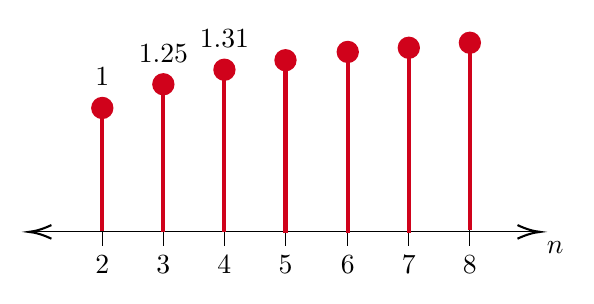
\begin{tikzpicture}[x=0.75pt,y=0.75pt,yscale=-1,xscale=1]
%uncomment if require: \path (0,412); %set diagram left start at 0, and has height of 412

%Straight Lines [id:da8584009914648288] 
\draw    (419.71,195) -- (177.29,195) ;
\draw [shift={(175.29,195)}, rotate = 360] [color={rgb, 255:red, 0; green, 0; blue, 0 }  ][line width=0.75]    (10.93,-3.29) .. controls (6.95,-1.4) and (3.31,-0.3) .. (0,0) .. controls (3.31,0.3) and (6.95,1.4) .. (10.93,3.29)   ;
\draw [shift={(421.71,195)}, rotate = 180] [color={rgb, 255:red, 0; green, 0; blue, 0 }  ][line width=0.75]    (10.93,-3.29) .. controls (6.95,-1.4) and (3.31,-0.3) .. (0,0) .. controls (3.31,0.3) and (6.95,1.4) .. (10.93,3.29)   ;
%Straight Lines [id:da9886964674804183] 
\draw    (299,189.29) -- (299,201.71) ;
%Straight Lines [id:da8156036240841317] 
\draw    (329,189.29) -- (329,201.71) ;
%Straight Lines [id:da7338901612135262] 
\draw    (358.42,189.29) -- (358.42,201.71) ;
%Straight Lines [id:da44762648985303743] 
\draw    (387.84,189.29) -- (387.84,201.71) ;
%Straight Lines [id:da9635121855917483] 
\draw    (269.58,189.29) -- (269.58,201.71) ;
%Straight Lines [id:da9816533416924345] 
\draw    (240.16,189.29) -- (240.16,201.71) ;
%Straight Lines [id:da026365304419259328] 
\draw    (210.74,189.29) -- (210.74,201.71) ;
%Straight Lines [id:da36890566565614835] 
\draw [color={rgb, 255:red, 208; green, 2; blue, 27 }  ,draw opacity=1 ][line width=1.5]    (210.74,135.29) -- (210.74,194.71) ;
\draw [shift={(210.74,135.29)}, rotate = 90] [color={rgb, 255:red, 208; green, 2; blue, 27 }  ,draw opacity=1 ][fill={rgb, 255:red, 208; green, 2; blue, 27 }  ,fill opacity=1 ][line width=1.5]      (0, 0) circle [x radius= 4.36, y radius= 4.36]   ;
%Straight Lines [id:da7429942794858413] 
\draw [color={rgb, 255:red, 208; green, 2; blue, 27 }  ,draw opacity=1 ][line width=1.5]    (240.16,123.87) -- (240.16,195.29) ;
\draw [shift={(240.16,123.87)}, rotate = 90] [color={rgb, 255:red, 208; green, 2; blue, 27 }  ,draw opacity=1 ][fill={rgb, 255:red, 208; green, 2; blue, 27 }  ,fill opacity=1 ][line width=1.5]      (0, 0) circle [x radius= 4.36, y radius= 4.36]   ;
%Straight Lines [id:da27787186266965624] 
\draw [color={rgb, 255:red, 208; green, 2; blue, 27 }  ,draw opacity=1 ][line width=1.5]    (269.58,116.87) -- (269.58,195.29) ;
\draw [shift={(269.58,116.87)}, rotate = 90] [color={rgb, 255:red, 208; green, 2; blue, 27 }  ,draw opacity=1 ][fill={rgb, 255:red, 208; green, 2; blue, 27 }  ,fill opacity=1 ][line width=1.5]      (0, 0) circle [x radius= 4.36, y radius= 4.36]   ;
%Straight Lines [id:da3329910181884447] 
\draw [color={rgb, 255:red, 208; green, 2; blue, 27 }  ,draw opacity=1 ][line width=1.5]    (299,112.29) -- (299,195.71) ;
\draw [shift={(299,112.29)}, rotate = 90] [color={rgb, 255:red, 208; green, 2; blue, 27 }  ,draw opacity=1 ][fill={rgb, 255:red, 208; green, 2; blue, 27 }  ,fill opacity=1 ][line width=1.5]      (0, 0) circle [x radius= 4.36, y radius= 4.36]   ;
%Straight Lines [id:da15731918285032842] 
\draw [color={rgb, 255:red, 208; green, 2; blue, 27 }  ,draw opacity=1 ][line width=1.5]    (329,108.29) -- (329,195.71) ;
\draw [shift={(329,108.29)}, rotate = 90] [color={rgb, 255:red, 208; green, 2; blue, 27 }  ,draw opacity=1 ][fill={rgb, 255:red, 208; green, 2; blue, 27 }  ,fill opacity=1 ][line width=1.5]      (0, 0) circle [x radius= 4.36, y radius= 4.36]   ;
%Straight Lines [id:da49004574560078384] 
\draw [color={rgb, 255:red, 208; green, 2; blue, 27 }  ,draw opacity=1 ][line width=1.5]    (358.42,106.29) -- (358.42,195.71) ;
\draw [shift={(358.42,106.29)}, rotate = 90] [color={rgb, 255:red, 208; green, 2; blue, 27 }  ,draw opacity=1 ][fill={rgb, 255:red, 208; green, 2; blue, 27 }  ,fill opacity=1 ][line width=1.5]      (0, 0) circle [x radius= 4.36, y radius= 4.36]   ;
%Straight Lines [id:da8874563427293995] 
\draw [color={rgb, 255:red, 208; green, 2; blue, 27 }  ,draw opacity=1 ][line width=1.5]    (387.84,103.87) -- (387.84,194.29) ;
\draw [shift={(387.84,103.87)}, rotate = 90] [color={rgb, 255:red, 208; green, 2; blue, 27 }  ,draw opacity=1 ][fill={rgb, 255:red, 208; green, 2; blue, 27 }  ,fill opacity=1 ][line width=1.5]      (0, 0) circle [x radius= 4.36, y radius= 4.36]   ;

% Text Node
\draw (210.74,205.11) node [anchor=north] [inner sep=0.75pt]    {$2$};
% Text Node
\draw (240.16,205.11) node [anchor=north] [inner sep=0.75pt]    {$3$};
% Text Node
\draw (269.58,205.11) node [anchor=north] [inner sep=0.75pt]    {$4$};
% Text Node
\draw (299,205.11) node [anchor=north] [inner sep=0.75pt]    {$5$};
% Text Node
\draw (329,205.11) node [anchor=north] [inner sep=0.75pt]    {$6$};
% Text Node
\draw (358.42,205.11) node [anchor=north] [inner sep=0.75pt]    {$7$};
% Text Node
\draw (387.84,205.11) node [anchor=north] [inner sep=0.75pt]    {$8$};
% Text Node
\draw (423.71,198.4) node [anchor=north west][inner sep=0.75pt]    {$n$};
% Text Node
\draw (210.74,125.89) node [anchor=south] [inner sep=0.75pt]    {$1$};
% Text Node
\draw (240.16,114.47) node [anchor=south] [inner sep=0.75pt]    {$1.25$};
% Text Node
\draw (269.58,107.47) node [anchor=south] [inner sep=0.75pt]    {$1.31$};


\end{tikzpicture}

          \caption{Sketch of $y[n]$}
          \label{fig:1}
        \end{figure}

      \item 

        Per the time-shifting property, we know that:

        $$y[n]=x[n]*h[n]\to y_1[n]=y[n-3]=x[n-3]*h[n]$$

        Which gives us:

        $$\boxed{y_1[n]=\frac{4}{3}\left[ 1-\left( \frac{1}{4} \right)^{n-4} \right]\text{ for }n\geq 5}$$

      \item 

        Per the time-shifting property, we know that:

        $$y[n]=x[n]*h[n]\to y_2[n]=y[n-2]=x[n]*h[n-2]$$

        $$\boxed{y_2[n]=\frac{4}{3}\left[ 1-\left( \frac{1}{4} \right)^{n-3} \right]\text{ for }n\geq 4}$$

      \item 

        Per the time-shifting property, we know that:

        $$y[n]=x[n]*h[n]\to y_3[n]=y[n+1]=x[n-2]*h[n+3]$$

        $$\boxed{y_3[n]=\frac{4}{3}\left[ 1-\left( \frac{1}{4} \right)^{n} \right]\text{ for }n\geq 1}$$

    \end{enumerate}

  \item

    We may simplify analysis by using a tabulating method. Using this, we can see that:

    $$x=\left\{ 0, 1, 1, 1 \right\}$$
    $$h=\left\{ 0, 0, 0, 0, 0, 1, 1, 1, 1, 1, 1 \right\}$$

    This can be written as:

    \begin{center}
    \begin{tabular}[H]{c|cccc}
      & 0 & 1 & 1 & 1\\
      \hline
      0 & \iddots & \iddots & \iddots & \iddots \\
      0 & \iddots & \iddots & \iddots & \iddots \\
      0 & \iddots & \iddots & \iddots & \iddots \\
      0 & \iddots & \iddots & \iddots & \iddots \\
      0 & \iddots & \iddots & \iddots & \iddots \\
      1 & \iddots & \iddots & \iddots & \iddots \\
      1 & \iddots & \iddots & \iddots & \iddots \\
      1 & \iddots & \iddots & \iddots & \iddots \\
      1 & \iddots & \iddots & \iddots & \iddots \\
      1 & \iddots & \iddots & \iddots & \iddots \\
      1 & \iddots & \iddots & \iddots & \iddots \\
    \end{tabular}
    \end{center}

    Here, we multiply the corresponding terms to populate the table:

    \begin{center}
    \begin{tabular}[H]{c|cccc}
      & 0 & 1 & 1 & 1\\
      \hline
      0 & 0 & 0 & 0 & 0\\
      0 & 0 & 0 & 0 & 0\\
      0 & 0 & 0 & 0 & 0\\
      0 & 0 & 0 & 0 & 0\\
      0 & 0 & 0 & 0 & 0\\
      1 & 0 & 1 & 1 & 1 \\
      1 & 0 & 1 & 1 & 1 \\
      1 & 0 & 1 & 1 & 1 \\
      1 & 0 & 1 & 1 & 1 \\
      1 & 0 & 1 & 1 & 1 \\
      1 & 0 & 1 & 1 & 1 \\
    \end{tabular}
    \end{center}

    Now we add diagonals to find the product, which gives us:

    $$y[n]=\{ 0, (0+0), (0+0+0), (0+0+0+0), (0+0+0+0), $$
    $$(0+0+0+0), (0+0+1+0), (0+1+1+0), $$
    $$(0+1+1+1), (0+1+1+1), (0+1+1+1),(1+1+1), (1+1), 1 \}$$

    This can be simplifed to:

    $$y[n]=\left\{ 0, 0, 0, 0, 0, 0, 1, 2, 3, 3, 3, 3, 2, 1, 0\cdots\right\}$$

    Using the step function notation, we may write:

    $$y[n]=u[n-6]+u[n-7]+u[n-8]-u[n-12]-u[n-13]-u[n-14]$$

  \item

    We can use a method similar to question (4) to find $N$. Let us begin with a table:

    \begin{center}
      \begin{tabular}[H]{c|cccccc}
        & 1 & 1 & 1 & 1 & 1 & 1 & 1\\
        \hline
        1 & & & & & & & \\
        \vdots & & & & & & & \\
      \end{tabular}
    \end{center}

    Using the tabulating method, we know that, for there to be a value of $4$, $h[n]$ needs to exist for at least 4 different $n$. Therefore, let us begin with the minimum such value for $h[n]$, when $N=3$, which gives us the following table:

    \begin{center}
      \begin{tabular}[H]{c|cccccc}
        & 1 & 1 & 1 & 1 & 1 & 1 \\
        \hline
        1 & 1 & 1 & 1 & 1 & 1 & 1\\
        1 & 1 & 1 & 1 & 1 & 1 & 1\\
        1 & 1 & 1 & 1 & 1 & 1 & 1 \\
        1 & 1 & 1 & 1 & 1 & 1 & 1 \\
      \end{tabular}
    \end{center}

    This gives us $y[n]=\left\{  1, 2, 3, 4, 4, 4, 3, 2, 1, 0, \cdots\right\}$. With this result, we see that $y[3]=4$, and $y[9]=0$. Thus, we find that:

    $$\boxed{N=3}$$

  \item

    \begin{enumerate}

      \item We can express this as $x_1[n]=u[n-3]$

        Since this is an LTI system, we know that the output will be shifted by the same amount (shifting property), which gives us:

        $$\boxed{x_1[n]\to y_1[n]=\left( \frac{1}{4} \right)^{n-3}u[n-3]-\left( \frac{1}{4} \right)^{n-4}u[n-4]}$$

      \item This input can be expressed as: $x_2[n]=u[n]-u[n-4]$

        Once again by the shifting property, as well as by homogeneity and superposition, we can write:

        $$\boxed{x_2[n]\to y_2[n]=\left( \frac{1}{4} \right)^{n}u[n]-\left( \frac{1}{4} \right)^{n-1}u[n-1]-\left( \frac{1}{4} \right)^{n-4}u[n-4]+\left( \frac{1}{4} \right)^{n-5}u[n-5]}$$

      \item This input can be expressed as: $x_3[n]=2u[n]-2u[n-1]$

        By the shifting, homogenous, and superposition principles of LTI systems, we get:

        $$x_3[n]\to y_2[n]=2\left( \frac{1}{4} \right)^{n}u[n]-2\left( \frac{1}{4} \right)^{n-1}u[n-1]-2\left( \frac{1}{4} \right)^{n-1}u[n-1]+2\left( \frac{1}{4} \right)^{n-2}u[n-2]$$

        Which can be simplifed:

        $$\boxed{x_3[n]\to y_2[n]=2\left( \frac{1}{4} \right)^{n}u[n]-4\left( \frac{1}{4} \right)^{n-1}u[n-1]+2\left( \frac{1}{4} \right)^{n-2}u[n-2]}$$

    \end{enumerate}

  \item

    Per convolution properties, we know:

    $$x(t)*\delta(t-t_o)\Rightarrow x(t-t_o)$$

    Thus, looking at the input, in addition to the fact that this is an LTI system, we can write:

    $$\boxed{y(t)=x(t)*h(t)\to y(t)=x(t+2)-2x(t)}$$

    Plotting this shift, we get:

    \begin{figure}[H]
      \centering
      \tikzset{every picture/.style={line width=0.75pt}} %set default line width to 0.75pt        

\begin{tikzpicture}[x=0.75pt,y=0.75pt,yscale=-1,xscale=1]
%uncomment if require: \path (0,863); %set diagram left start at 0, and has height of 863

%Shape: Axis 2D [id:dp009613639780450267] 
\draw  (265,542.1) -- (508,542.1)(289.3,345) -- (289.3,564) (501,537.1) -- (508,542.1) -- (501,547.1) (284.3,352) -- (289.3,345) -- (294.3,352)  ;
%Shape: Axis 2D [id:dp33103048834679427] 
\draw  (313.6,542.1) -- (70.6,542.1)(289.3,345) -- (289.3,564) (77.6,537.1) -- (70.6,542.1) -- (77.6,547.1) (294.3,352) -- (289.3,345) -- (284.3,352)  ;
%Straight Lines [id:da34018245844871986] 
\draw    (223.88,536.68) -- (223.88,542.1) ;
%Straight Lines [id:da03268958320957127] 
\draw    (223.88,542.1) -- (223.88,547.52) ;
%Straight Lines [id:da019398181529335923] 
\draw    (158.46,542.1) -- (158.46,547.52) ;
%Straight Lines [id:da4734553575991777] 
\draw    (158.46,536.68) -- (158.46,542.1) ;
%Straight Lines [id:da8561932810123746] 
\draw    (354.72,542.1) -- (354.72,547.52) ;
%Straight Lines [id:da15564111396343616] 
\draw    (354.72,536.68) -- (354.72,542.1) ;
%Straight Lines [id:da25447006785528636] 
\draw    (420.14,542.1) -- (420.14,547.52) ;
%Straight Lines [id:da14653617720880696] 
\draw    (420.14,536.68) -- (420.14,542.1) ;
%Shape: Axis 2D [id:dp5465647021447075] 
\draw  (313.6,542.1) -- (70.6,542.1)(289.3,739.2) -- (289.3,520.2) (77.6,547.1) -- (70.6,542.1) -- (77.6,537.1) (294.3,732.2) -- (289.3,739.2) -- (284.3,732.2)  ;
%Shape: Axis 2D [id:dp14692899284555505] 
\draw  (265,542.1) -- (508,542.1)(289.3,739.2) -- (289.3,520.2) (501,547.1) -- (508,542.1) -- (501,537.1) (284.3,732.2) -- (289.3,739.2) -- (294.3,732.2)  ;
%Straight Lines [id:da5562490218389332] 
\draw    (294.72,607.52) -- (289.3,607.52) ;
%Straight Lines [id:da04132983908633392] 
\draw    (289.3,607.52) -- (283.88,607.52) ;
%Straight Lines [id:da3128638973663658] 
\draw    (294.72,672.94) -- (289.3,672.94) ;
%Straight Lines [id:da07301602070698754] 
\draw    (289.3,672.94) -- (283.88,672.94) ;
%Straight Lines [id:da7936618811135429] 
\draw    (294.72,640.23) -- (289.3,640.23) ;
%Straight Lines [id:da1328467197459401] 
\draw    (289.3,640.23) -- (283.88,640.23) ;
%Straight Lines [id:da6061062079163653] 
\draw    (294.72,574.81) -- (289.3,574.81) ;
%Straight Lines [id:da8698562775451101] 
\draw    (289.3,574.81) -- (283.88,574.81) ;
%Straight Lines [id:da653612280129497] 
\draw    (295.72,441.52) -- (290.3,441.52) ;
%Straight Lines [id:da0578746791058401] 
\draw    (295.72,506.94) -- (290.3,506.94) ;
%Straight Lines [id:da5836257479573154] 
\draw    (295.72,474.23) -- (290.3,474.23) ;
%Straight Lines [id:da5214729231831259] 
\draw    (295.72,408.81) -- (290.3,408.81) ;
%Straight Lines [id:da6490663694872785] 
\draw    (288.72,441.52) -- (283.3,441.52) ;
%Straight Lines [id:da1853875758047513] 
\draw    (288.72,506.94) -- (283.3,506.94) ;
%Straight Lines [id:da07012480530135812] 
\draw    (288.72,474.23) -- (283.3,474.23) ;
%Straight Lines [id:da049298153511061815] 
\draw    (288.72,408.81) -- (283.3,408.81) ;
%Straight Lines [id:da2797673259319313] 
\draw [color={rgb, 255:red, 74; green, 144; blue, 226 }  ,draw opacity=1 ][line width=1.5]    (158.3,506.94) -- (158.46,542.1) ;
%Straight Lines [id:da9171226989948468] 
\draw [color={rgb, 255:red, 74; green, 144; blue, 226 }  ,draw opacity=1 ][line width=1.5]    (224.01,474.23) -- (158.3,506.94) ;
%Straight Lines [id:da5374617282022399] 
\draw [color={rgb, 255:red, 74; green, 144; blue, 226 }  ,draw opacity=1 ][line width=1.5]    (223.88,474.39) -- (223.59,506.94) ;
%Straight Lines [id:da7848730881640463] 
\draw [color={rgb, 255:red, 74; green, 144; blue, 226 }  ,draw opacity=1 ][line width=1.5]    (289.3,542.1) -- (223.59,506.94) ;
%Straight Lines [id:da8672470342925992] 
\draw [color={rgb, 255:red, 74; green, 144; blue, 226 }  ,draw opacity=1 ][line width=1.5]    (289.3,542.1) -- (289.3,607.52) ;
%Straight Lines [id:da13551389878098385] 
\draw [color={rgb, 255:red, 74; green, 144; blue, 226 }  ,draw opacity=1 ][line width=1.5]    (289.3,607.52) -- (354.72,672.94) ;
%Straight Lines [id:da6021136280695535] 
\draw [color={rgb, 255:red, 74; green, 144; blue, 226 }  ,draw opacity=1 ][line width=1.5]    (420.14,542.1) -- (354.72,607.52) ;
%Straight Lines [id:da8971838941380121] 
\draw [color={rgb, 255:red, 74; green, 144; blue, 226 }  ,draw opacity=1 ][line width=1.5]    (354.72,607.52) -- (354.72,672.94) ;

% Text Node
\draw (287.3,545.5) node [anchor=north east] [inner sep=0.75pt]    {$0$};
% Text Node
\draw (223.88,550.92) node [anchor=north] [inner sep=0.75pt]    {$-1$};
% Text Node
\draw (158.46,550.92) node [anchor=north] [inner sep=0.75pt]    {$-2$};
% Text Node
\draw (354.72,550.92) node [anchor=north] [inner sep=0.75pt]    {$1$};
% Text Node
\draw (420.14,550.92) node [anchor=north] [inner sep=0.75pt]    {$2$};
% Text Node
\draw (281.88,574.81) node [anchor=east] [inner sep=0.75pt]    {$-1$};
% Text Node
\draw (281.88,607.52) node [anchor=east] [inner sep=0.75pt]    {$-2$};
% Text Node
\draw (281.88,640.23) node [anchor=east] [inner sep=0.75pt]    {$-3$};
% Text Node
\draw (281.88,672.94) node [anchor=east] [inner sep=0.75pt]    {$-4$};
% Text Node
\draw (281.3,506.94) node [anchor=east] [inner sep=0.75pt]    {$1$};
% Text Node
\draw (281.3,474.23) node [anchor=east] [inner sep=0.75pt]    {$2$};
% Text Node
\draw (281.3,441.52) node [anchor=east] [inner sep=0.75pt]    {$3$};
% Text Node
\draw (281.3,408.81) node [anchor=east] [inner sep=0.75pt]    {$4$};
% Text Node
\draw (289.72,337) node [anchor=south] [inner sep=0.75pt]    {$y( t)$};
% Text Node
\draw (510,533.4) node [anchor=north west][inner sep=0.75pt]    {$t$};


\end{tikzpicture}

      \caption{Plot for $y(t)=x(t+2)-2x(t)$}
      \label{fig:2}
    \end{figure}

  \item

    \begin{enumerate}

      \item Using this, we can rewrite $x$ as:

        $$x(t)=u(t)-u(t-1)$$

        Which would make $h$:

        $$h(t)=u(t-2)-u(t-4)$$

        This gives us:

        $$y(t)=\int[u(t)-u(t-1)]*[u(t-2)-u(t-4)]\,dt$$

        Which expands to:

        $$y(t)=\int u(t)u(t-2)-u(t)u(t-4)-u(t-1)u(t-2)+u(t-1)u(t-4)\,dt$$

        To analyze, we can use the following properties:

        $$r(t)*r(t-T_1)=r(t-T_1)$$
        $$r(t-T_1)*r(t-T_2)=r(t-T_1-T_2)$$

        This gives us:

        $$y(t)=r(t-2)-r(t-4)-r(t-3)+r(t-5)$$
        $$\boxed{y(t)=r(t-2)-r(t-3)-r(t-4)+r(t-5)}$$

        And the plot becomes:

        \begin{figure}[H]
          \centering
          \tikzset{every picture/.style={line width=0.75pt}} %set default line width to 0.75pt        

\begin{tikzpicture}[x=0.75pt,y=0.75pt,yscale=-1,xscale=1]
%uncomment if require: \path (0,863); %set diagram left start at 0, and has height of 863

%Shape: Axis 2D [id:dp009613639780450267] 
\draw  (265,542.1) -- (508,542.1)(289.3,345) -- (289.3,564) (501,537.1) -- (508,542.1) -- (501,547.1) (284.3,352) -- (289.3,345) -- (294.3,352)  ;
%Straight Lines [id:da8561932810123746] 
\draw    (354.72,542.1) -- (354.72,547.52) ;
%Straight Lines [id:da15564111396343616] 
\draw    (354.72,536.68) -- (354.72,542.1) ;
%Straight Lines [id:da25447006785528636] 
\draw    (420.14,542.1) -- (420.14,547.52) ;
%Straight Lines [id:da14653617720880696] 
\draw    (420.14,536.68) -- (420.14,542.1) ;
%Straight Lines [id:da653612280129497] 
\draw    (295.72,441.52) -- (290.3,441.52) ;
%Straight Lines [id:da0578746791058401] 
\draw    (295.72,506.94) -- (290.3,506.94) ;
%Straight Lines [id:da5836257479573154] 
\draw    (295.72,474.23) -- (290.3,474.23) ;
%Straight Lines [id:da5214729231831259] 
\draw    (295.72,408.81) -- (290.3,408.81) ;
%Straight Lines [id:da6490663694872785] 
\draw    (288.72,441.52) -- (283.3,441.52) ;
%Straight Lines [id:da1853875758047513] 
\draw    (288.72,506.94) -- (283.3,506.94) ;
%Straight Lines [id:da07012480530135812] 
\draw    (288.72,474.23) -- (283.3,474.23) ;
%Straight Lines [id:da049298153511061815] 
\draw    (288.72,408.81) -- (283.3,408.81) ;
%Straight Lines [id:da9171226989948468] 
\draw [color={rgb, 255:red, 74; green, 144; blue, 226 }  ,draw opacity=1 ][line width=1.5]    (354.43,508.55) -- (321.72,542.1) ;
%Straight Lines [id:da5374617282022399] 
\draw [color={rgb, 255:red, 74; green, 144; blue, 226 }  ,draw opacity=1 ][line width=1.5]    (420.14,542.1) -- (499,542) ;
%Straight Lines [id:da6844813610272923] 
\draw    (321.72,535.68) -- (321.72,541.1) ;
%Straight Lines [id:da7346761603367431] 
\draw    (387.14,535.68) -- (387.14,541.1) ;
%Straight Lines [id:da6462550276222756] 
\draw    (321.72,541.1) -- (321.72,546.52) ;
%Straight Lines [id:da7832405233466256] 
\draw    (387.14,541.1) -- (387.14,546.52) ;
%Straight Lines [id:da9300431401294764] 
\draw [color={rgb, 255:red, 74; green, 144; blue, 226 }  ,draw opacity=1 ][line width=1.5]    (386.85,508.55) -- (354.43,508.55) ;
%Straight Lines [id:da7495999047891863] 
\draw [color={rgb, 255:red, 74; green, 144; blue, 226 }  ,draw opacity=1 ][line width=1.5]    (420.41,541.26) -- (386.85,508.55) ;
%Straight Lines [id:da8437892531840325] 
\draw [color={rgb, 255:red, 74; green, 144; blue, 226 }  ,draw opacity=1 ][line width=1.5]    (289.3,542.1) -- (321.72,541.1) ;

% Text Node
\draw (321.72,549.92) node [anchor=north] [inner sep=0.75pt]    {$2$};
% Text Node
\draw (354.72,550.92) node [anchor=north] [inner sep=0.75pt]    {$3$};
% Text Node
\draw (281.3,506.94) node [anchor=east] [inner sep=0.75pt]    {$1$};
% Text Node
\draw (281.3,474.23) node [anchor=east] [inner sep=0.75pt]    {$2$};
% Text Node
\draw (281.3,441.52) node [anchor=east] [inner sep=0.75pt]    {$3$};
% Text Node
\draw (281.3,408.81) node [anchor=east] [inner sep=0.75pt]    {$4$};
% Text Node
\draw (289.72,337) node [anchor=south] [inner sep=0.75pt]    {$y( t)$};
% Text Node
\draw (510,533.4) node [anchor=north west][inner sep=0.75pt]    {$t$};
% Text Node
\draw (387.14,549.92) node [anchor=north] [inner sep=0.75pt]    {$4$};
% Text Node
\draw (420.14,550.92) node [anchor=north] [inner sep=0.75pt]    {$5$};


\end{tikzpicture}

          \caption{Plot for $y(t)=r(t-2)-r(t-3)-r(t-4)+r(t-5)$}
          \label{fig:3}
        \end{figure}

      \item 

        We can determine $\frac{d}{dt}[y(t)]$ to be:

        $$\frac{d}{dt}[y(t)]=u(t-2)-u(t-3)-u(t-4)+u(t-5)$$

        The discontinuities may be identified by differentiating again to get:

        $$\frac{d^2}{dt^2}[y(t)]=\delta(t-2)-\delta(t-3)-\delta(t-4)+\delta(t-5)$$

        We know that each impulse represents a discontinuity; Therefore, we can tell that there are 4 discontinuities, at $t=2,3,4,$ and $5$, for $d/dt[y(t)]$

    \end{enumerate}

  \item

    \begin{enumerate}

      \item 

        We know that the impulse response can be determined if $x(t)=\delta(t)$:

        $$y(t)=\int_{-\infty}^{t}e^{-(t-\tau)}x(\tau-2)\,d\tau$$
        $$y(t)=\int_{-\infty}^{t}e^{-(t-\tau)}\delta(\tau-2)\,d\tau$$

        We also know from the property of the impulse that:

        $$\int_{-\infty}^{\infty} x(t)\delta(t-t_o)\,dt=x(t_o)$$

        Thus, we can see that:

        $$\boxed{h(t)=e^{-(t-2)}}$$

      \item 

        We may begin by writing $x(t)$:

        $$x(t)=u(t+1)-u(t-2)$$

        Alternatively, this may be written in laplace form as:

        $$x(s)=\frac{e^s}{s}-\frac{e^{-2s}}{s+1}$$

        Which gives us:

        $$h(s)=\frac{1}{s+1}$$

        Multiplying the two togetherm, we get:

        $$x(s)h(s)=e^s\left[ \frac{1}{s}-\frac{1}{s+1} \right]-\frac{e^{-2s}}{(s+1)^2}$$

        We then take the inverse laplace transform to finally find:

        $$\boxed{y(t)=u(t+1)-e^{-t-1}u(t+1)-(t-2)e^{2-t}u(t-2)}$$

        $$$$

    \end{enumerate}

\end{enumerate}

\end{document}

